%\documentclass[a4paper]{article}
\documentclass[a4paper, 12pt]{article}

\usepackage[english]{babel}
\usepackage[utf8]{inputenc}
\usepackage{amsmath}
\usepackage{graphicx}
\usepackage{epsfig}
\usepackage[colorinlistoftodos]{todonotes}
\usepackage[hidelinks]{hyperref}
\usepackage[margin=1in]{geometry}

\usepackage{tikz}
\usepackage{pgfplots}
\usetikzlibrary{shapes}



\usepackage{setspace}
\doublespacing

%\usepackage{Times} %or \usepackage{mathptmx}
%\documentclass[a4paper,12pt]{report}

\title{STELLAR ROTATION}

\author{TIMOTHY HOLMES \\ 
        DePaul University}

\date{\today}

\newcommand{\gfigure}[4]
{
	\begin{figure}
      \begin{center}
          \includegraphics[#3]{#4}
          \caption{#1}
          \label{Figure:#2}
      \end{center}
    \end{figure}
}
\newcommand{\figref}[1]{Figure~\ref{Figure:#1}}

\begin{document}
\maketitle

\begin{abstract}
The study of stellar rotation is an important due to all the implications this process has on a star. There are several measurement techniques used to measure a stars rotation. Newer technology has brought fourth newer techniques which has ultimately lead to better predictive models. These models are used to test against observational data. The models are setup where a star is simulated to have no rotation, this is compared against observational data. Several findings show that rotation affects the structure, evolution and lifespan, and nucleosynthesis of a star. 
\end{abstract}

\begin{center}
\section{INTRODUCTION}
\end{center}

Mankind has had evidence of stellar rotation since the days of Galileo. In the late nineteenth century and early twentieth century, astronomers started to use spectroscopy to measure the rotation of stars. Earlier modern studies between the 1960's and 1980's focused on projected rotational velocities. The 1990's allowed for the study of complete rotational period distributions for a magnitude of low-mass stars in the Pre-Main Sequence (PMS) and Main Sequence (MS). While more recent studies have concentrated on the angular momentum (AM) evolution of cool stars is strongly mass dependent. 
The evolution of a star that rotates starts long before a star forms. In fact, the star at formation impact the evolution of the star.

\begin{center}
\section{PROCEDURES}
\end{center}

The first paper "Observational Studies of Stellar Rotation". The author in this paper went over the history of stellar rotation, measuring techniques and current research efforts. Highlighting the paper "Stellar Differential Rotation and Coronal Timescales". The authors of this paper investigated the timescales of evolution of the stellar coronae and the response to the surface differential rotation. Referencing the paper "Rotation of planet-harbouring stars". The author went into detail to describe the effects of stellar rotation while planets orbit the star, much like our own. Introducing the paper "Impact of rotation on stellar models". The authors of this paper also explain the impacts of how the angular moment will impact certain features of the star over the stars lifespan. The final paper "Influence of rotation on Stellar Evolution". In this paper the author targeted the impacts that rotation has on the star. To give evidence, the author provided models that began to describe the impacts such as internal structure, nucleosynthesis and global evolution of stars.

\begin{center}
\section{DISCUSSION}
\end{center}

In order to fully understand why stellar objects rotate, it is important to understand the evolution of star formation. Prior to star formation, there are some parts in space that have densely populated regions with various kinds of matter. The interest in star formation involves molecular clouds. These molecular clouds are turbulent and their average velocity is dependent upon rotation. When the cloud eventually becomes dense enough and the cloud does not pull itself apart from its velocity, the cloud will eventually experience gravitational collapse. While the effect of the collapse exhausts a portion of the total angular momentum, the newly formed star will still inherit a portion of the former clouds angular momentum. Given the nature of how a star forms, it is improbable that a star could from without presence of angular momentum. Thus, a rotating star is the most probable scenario throughout the Universe. Throughout this section, the measuring methods, impacts and influence, and recent studies are highlighted.

\subsection{Measuring Methods}

There is a vast array of measurement techniques used to determine a variation of quantities and applications for determining rotation in a star. Measurements for this physical phenomenon include: photometry, spectroscopy, spectropolarimetry, sismology and interferometry. The various measurements are talked about in depth below.

\subsubsection{Photometry}

Photometry is the oldest method that is used to measure stellar rotation. This specific method is what Galileo used to observe stellar rotation, it is simply the monitoring of magnetic spots on the stars surface. Simply put, it is the light curve modulation by rotation that allows for rotation periods to be found. This technique has an advantage over spectroscopy by being free of geometric effects and the ability of easily converting the period to angular velocity. In today's research, this approach is still being used by satellites that capture data over large timescales. The target stars for this measurement are stars that are magnetically active and have spots on the surface. 

\subsubsection{Spectroscopy}

The Spectroscopy method uses spectral lines broadening that occurs due to surface rotation. An estimated projected surface velocity on the line of sight can be obtained from this method. This is a powerful technique that allows for measurements of what are known as fast spinner, stars that rotate above $30 \; km \; s^{-1}$. However, this method is not as adequate when measuring slow rotating star, stars that rotate under $20 \; km \; s^{-1}$. A method called cross-correlation analysis is better for determining the rotation for a slow star. 

\subsubsection{spectropolarimetry}
Spectropolarimetry as well as doppler imaging will of polarized light from the rotation gives the periods of rotations and surface latitudinal differential rotation.

\subsubsection{Sismology}
Oscillation modes from a rotating star give a rotation profile. 

\subsubsection{Interferometry}

By directly imaging the rapidly rotating non-spherical stellar surface, a mean rotation rate can be discovered. Essentially, the star is rotating rapidly in such a way that it deforms the star. Since the ratio between the equatorial to the polar radii can be measured, the deformity can be calculated. This means that the star will have to be rotating close to its critical velocity. This method is in fact very similar to spectroscopy, so much so that both this technique and the spectroscopy technique can be combined.

After exploring all of the different methods of measurements, it is clear that not all measurements work far all stars. Different distances play a factor into what can and can not be measured. There is also the subject of if a stellar object takes on the shape of a sphere or the shape of a ellipsoid, also has an impact on the way a stellar object gets measured for rotation. These implications can severely limit what information can be pulled from a stellar object. The only star that has currently been measured using all the measurement techniques listed above is the Sun as mentioned in Figure 1. Also shown in Figure 1 is the quantity that is obtained by each technique. Highlighted in red it the unique quantity obtained by each specific measurement. This info-graph also repeats the stars applicable, the limitations, and the instruments used for each measurement technique. 

\subsection{Impacts and Influence of Rotation}

It would be very rare and unlikely for a star not to rotate due to the nature and formation of them. The evolution of star formation was discussed in the beginning of this chapter. There are inherently immense causes for concern when thinking about the effect of a rotating star. Dependent upon the angular velocity, mass, and other physical properties, are just a few things that have affects on stars. The rotation could could be a contributing factor that alters the structure, evolution, and nucleosynthesis of stars. If this claim is true, with conception and observation, does the angular momentum have these lasting impacts. If there is a correlation, then to what extent does angular rotation impact a stellar object. In order to discover the influence that rotation might have on a star, models are created to mimic the stars activity. From here the models are run with the condition that there is no rotation from the star. The information and data provided from this model is then compared to what is observed to a similar star in the Universe. This comparison is an attempt to find out conceptually what the effects of rotation do to the star. From the paper "Impact of rotation on stellar models" and "
Influence of Rotation on Stellar Evolution"  a few key concepts are discovered and discussed. 

When considering the rotation of a star, one significant and notable affect comes from the magnetic field. Magnetic fields in a star have enough influence to affect the rotation. The magnetic field also brings up another important topic that is referred to as magnetic breaking. This occurs when the material composing the stellar winds are funneled along magnetic lines. It is often thought to keep starts from breaking apart in the early life of a star. There are two specific models that are popular when considering the affects of the magnetic field. The first is the shear models and the other is the radiative-dyamo models [4]. The first model focuses on the core rotating a few times faster than the envelope. While the second model focuses on a solid body rotation. During the PMS without magnetic breaking, both models predicted different outputs. The Sears model had predicted that the breaking affect had the impact of boosting  the chemical enrichment inside the star while the surface had no breaking. While the radiative-dynamo models had the breaking slow down and the surface enrichment decreased. 

Another rotational factor changes the evolution of the star, in this instance, it is thought that rotation has an impact on a stars lifetime. The image Figure 2. in the Appendix displays isochrones for different aged stars. It should be noted that an isochrone is just a population of same aged stars. The different colored lines represent the different age groups. The shear model without breaking found that the different aged groups were more scattered when rotation was not considered.

Stars that harness planets in their orbit, like the Sun, also show affects on the rotation of stars. In the star formation phase, it is the planets in the vicinity that help the stars form. Therefore, in the earliest stage of star evolution, planets contribute to the braking process and in return stars have a better chance of survival. Tidal forces from a planet produce an exchange of angular momentum between the orbit of a planet and the star. The transfer of angular momentum can speed up a planets orbit and can slow it down. Depending on what the planet will do, the star's rotation will do the opposite. 

The paper "Rotation of planet-harbouring stars" goes in depth on the affects of a stars rotation with plants present, while the paper "Impact of rotation on stellar models" briefly touches on the fact that this planets disrupt a stars rotation. The influence of plants on a stars rotation go like this, if a planet's orbital period matches the stars rotational period then there are no affects to the rotation. This is known as synchronous rotation. However, if anything not equal is subject to affect the rotation as previously explained. The paper demonstrates planet's in this paper with massive exoplanets in close orbits, but refers to them as hot Jupiter. Therefore, through the rest of this section, it is now defined. Another scenario involves the hot Jupiter systems having angular momentum lost from the orbit of the plant resulting in the "spin-up" of the star, this ultimately kills the planet. This spin-up affect leads to an increase in magnetic field and increases the magnetic braking affect. Hot Jupiter's can also modify the structural integrity of a star and change the course of stellar winds. When the stellar wind changes, the efficiency of magnetic stellar wind breaking diminishes. This type of scenario is referred to as a spin-down and would now increase the rate of rotation. 

Finally, one of the last areas of affects on stellar rotation come in the early chemical evolution of stars or the process of nucleosynthesis, The implications of a fast rotator is decreased metallicity, the faster a star rotates the faster the metallicity decreases. The other implication involves rotational mixing, this becomes more efficient at low metallicity. The mixing process when matter exchanges from H-burning to He-burning increases the rotation of the star.

\subsection{Differential Rotation}

One final topic involved the chaotic rotations that occur in a star. Differential rotation is observed when angular velocities vary with latitude. When the angular velocity decreases while the latitude increases, this signals a differential rotation. This occurs due to a stars turbulent convection within the star. Since convection carries energy from the center of the star outward to the surface of the star. 

In the final paper "Stellar Differential Rotation and Coronal Timescales", a recent study investigates the timescales of evolution of stellar coronae from the surface differential rotation. 

The coronae, which is the layer of plasma that surrounds the stars on the surface. The coronae has a dynamic response to surface flux transport from the star's magnetic field. This transport has an associated timescale that vary from relatively short time scales of differential rotation and flux transport to long timescales of stellar cycles. The surface dynamics of a star include X-ray luminosity, stellar wind, coronal mass ejections and flares. Some of these topics have been addressed previously in other sections of this paper. The Sun's coronal structure and dynamics are well studied and understood. The translation of findings to other stars is quite difficult to do. 

Evidence provided shows that many stars have higher levels of differential rotation than the Sun. Due to this observation, it is important to understand how enhanced differential rotation affects the dynamics of the stellar corona. In this recent study, the authors used a magnetic flux transport model to determine the evolution of the stellar phosphoric field. This is used to then derive the evolution of the coronal magnetic field, applying a magnetofrictional technique.

The model used was a simulated portion of a stellar corona. Using a spherical coordinate system with $r$ as the distance to the center of the star, $\theta$ the co-latitude, and $\phi$ the azimuthal angle. The study simulated the stellar corona between $0^{\circ}$ and $140^{\circ}$ longitude, $-4.5^{\circ}$ and $65^{\circ}$ latitude and a radius between $1 \; R_{\odot}$ and $2.5 \; R_{\odot}$. From the model the authors were able to use the surface flux transport model to prescribe the evolution of the phosphoric magnetic field, coupled with magnetofrictional technique to determine the evolution of the coronal magnetic field. The authors found that the formation timescale of a flux rope is roughly proportional to the geometric mean of the equator-pole lap time and the surface diffusion timescale. This means that this short life time is brought upon by the enhanced diffusion weakening the field. And stars with high differential rotation may have a high dynamical coronae. This result makes sense for one reason. If the stars rotation is differential, meaning chaotic and turbulent, then the affects of this turbulent rotation should be seen through the star. The turbulent occurrence will have the affect of making other attributes of the star also chaotic, such as the magnetic field for one example. The dynamical coronae observed in this study must be caused by the differential nature of the stars rotation. 

\begin{center}
\section{CONCLUSIONS}
\end{center}

In conclusion, the rotation of a star actually come long before a star is born. The rotation of a star comes in the phase of star evolution. One the molecular cloud collapses, the star captures a fraction of the angular momentum the molecular cloud once had. Measuring the rotation of a star predates Galileo and there are many different ways to observe the rotation of a star. Each technique varies in application, instrumentation, accuracy, measured quantity and limitations. Above all, all methods are useful methods with a different purpose. The presence of external forces and objects can have an affect on the rotation of a star. Evidence shows that during the the impact of a stars rotation can have the most significant impact during the Pre-Main Sequence and during the Main Sequence. To observe these impacts, models are created to test against observed data to fully find the impacts on the star. The impacts on a star in its early life shows that if can have an impact on its lifespan, the rotational impacts can span from planetary affects to the nucleosynthesis process. More recent studies include more accurate models from observed data. Recent studies have advanced in depth models to simulate a stars coronae, magnetic field, and much more. From these advanced models astronomers have been able to better replicate the rotation and the more turbulent differential rotation found in stars with convection.  


\newpage

\begin{center}
\nocite{*}
\bibliographystyle{IEEEannot}
\bibliography{thesis}
\end{center}

\newpage

\begin{center}
\section{APPENDIX}
\end{center}

\begin{figure}[h]
    \centering
    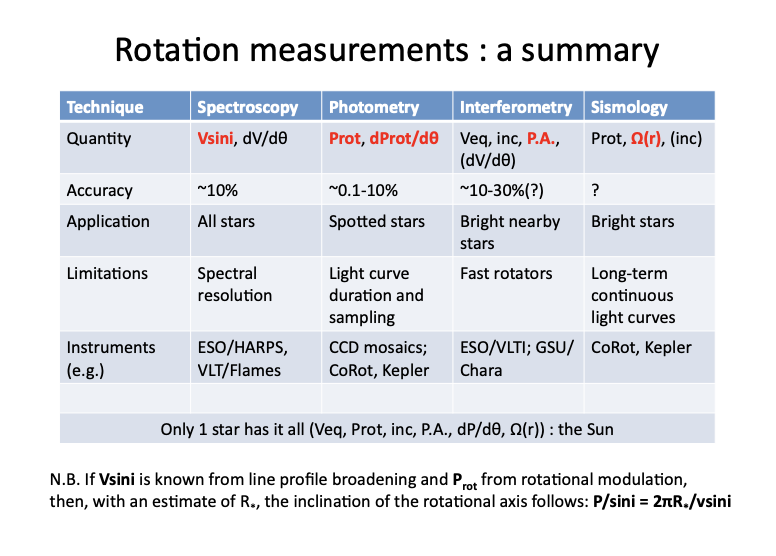
\includegraphics[width=0.5\textwidth]{fig2.png}
    \caption{Comparison of measurement techniques.}
    \label{fig:mesh1}
\end{figure}

\begin{figure}[h]
    \centering
    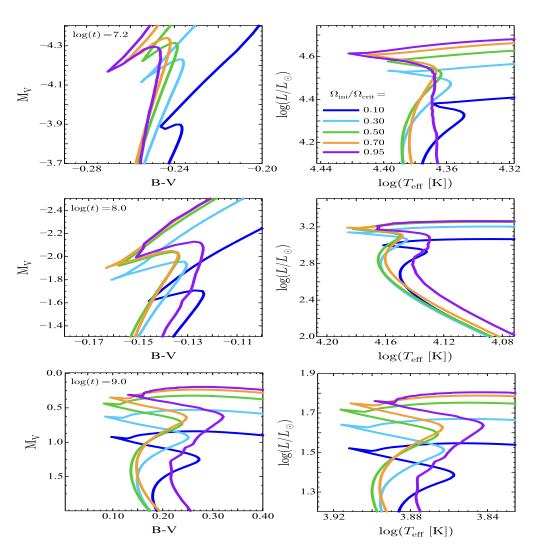
\includegraphics[width=0.5\textwidth]{fig1.png}
    \caption{Model of different aged clusters with no stellar rotation.}
    \label{fig:mesh1}
\end{figure}

\end{document}